\documentclass{article}
\usepackage{pgf,tikz,tikzscale} 
\usepackage{amssymb}
\usepackage{tcolorbox}
\usepackage{tkz-berge}
\usepackage{xcolor}
\usepackage[utf8]{inputenc}
\usepackage[english]{babel}
\usepackage{multicol}
\usepackage{enumerate}	
\usepackage{graphicx,lipsum,pgfplots} 
\usepackage{amsmath, amsthm}                 
\usepackage[top=1in,bottom=1in, left=1in, right=1in] {geometry}  
\usepackage{fancyhdr}       
\usepackage{blkarray}


\pagestyle{fancy}              
\lhead{Math 5563 \newline Graph Theory HW6, Ch9}   
\rhead{Warren Keil}







\begin{document}
\setlength{\parindent}{0cm}   %%%%%%%% KEEP THIS  for block style paragraphs. 



%\textbf{11a.}  Suppose \(G\) is a graph on \(n\leq5\) vertices such that \(G\) is not coplanar. Prove that \(G=K_5\) or \(G=K_5^c\). 


%\vspace{3mm}
%\textit{Proof.} Let \(G\) be a graph on \(n\leq5\) vertices such that \(G\) is not coplanar. 

\textbf{2a.} Compute the oriented vertex-edge incidence matrix \(Q=Q(G)\) corresponding to the oriented graph illustrated in the book. 


\vspace{3mm}
\textit{Solution.} \[
Q(G) = 
\begin{bmatrix}
1  &   0 &  0  & -1   &  1\\
 -1&	1&0	&0	&0	 \\
 0&-1	&	1&	0&	-1 \\
 0 &0	&	-1&	1&	0 \\
\end{bmatrix}
\]


\vspace{3mm}


\textbf{4a.} Let \(G\) be the graph illustrated in Figure 9.12 in the text. Find \(L(G)\). 

\vspace{3mm}
\textit{Solution.} To find \(L(G)\), we use the fact that \(L(G)\) is equal the the diagonal matrix containing the degrees of the vertices of \(G\) on the diagonal less the adjacency matrix of \(G\). 
\[
L(G) =  D(G) - A(G)
\]
Thus, listing labels of the vertices as the same order of the columns and rows, we get:
\begin{align*}
L(G) &=
\begin{bmatrix}
 4&0 &0 &0 & 0\\
  0&2 &0 & 0&0 \\
  0 & 0&3 & 0&0 \\
    0&0 & 0&3 &0 \\
     0&0 &0 & 0&2 \\
\end{bmatrix}-
\begin{bmatrix}
 0& 1&1 &1 & 1\\
  1& 0&1 &1 &0 \\
  1 &1 & 0&0 &1 \\
  1  &1 & 0& 0& 0\\
   1  & 0& 1& 0& 0\\
\end{bmatrix}\\
&=
\begin{bmatrix}
 4& -1&-1 &-1 & -1\\
  -1& 2&-1 &-1 &0 \\
  -1 &-1 & 3&0 &-1 \\
  -1  &-1 & 0& 3& 0\\
   -1  & 0& -1& 0& 2\\
\end{bmatrix}.
\end{align*}

\vspace{3mm}


\textbf{4c.} Illustrate all \(t(G)\) spanning trees of \(G\). 

\vspace{3mm}

\textit{Solution.} From page 178, we know \(t(G) = (-1)^{i+j} \det(L(G)_{ij}) \). And the matrix-tree theorem shows that this gives the number of spanning trees for a graph \(G\). Using mathematica, we find \(t(G)\) for the graph in the problem. 
\begin{verbatim}
In[3]:= G = {
  {2, -1, 0, 0},
  {-1, 3, -1, 0},
  {0, -1, 3, -1},
  {0, 0, -1, 2}
 }

Out[3]= {{2, -1, 0, 0}, {-1, 3, -1, 0}, {0, -1, 3, -1}, {0, 0, -1, 2}}
In[4]:= Det[G]

Out[4]= 21
\end{verbatim}
Thus, using mathematica, we find \(t(G)=21\). We will draw these 21 different spanning trees of the graph while possibly omitting isomorphic graphs. 
\newpage
\textbf{4c. continued} We now show examples of all 21 spanning trees of the graph in figure 9.12. 

\begin{center}
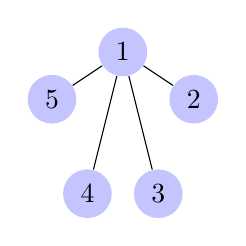
\begin{tikzpicture}
  [scale=.15,auto=left,every node/.style={circle,fill=blue!23}]
  \node (1) at (6,12) {1};
  \node (2) at (12,8)  {2};
  \node (3) at (9,0)  {3};
  \node (4) at (3,0)  {4};
  \node (5) at (0,8)  {5};
  
  \foreach \from/\to in { 1/5,1/4,1/3,1/2}
    \draw (\from) -- (\to);

\end{tikzpicture}\hspace{6mm}
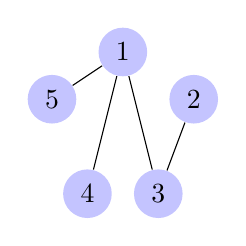
\begin{tikzpicture}
  [scale=.15,auto=left,every node/.style={circle,fill=blue!23}]
  \node (1) at (6,12) {1};
  \node (2) at (12,8)  {2};
  \node (3) at (9,0)  {3};
  \node (4) at (3,0)  {4};
  \node (5) at (0,8)  {5};
  
  \foreach \from/\to in {1/5,1/4,1/3,3/2}
    \draw (\from) -- (\to);

\end{tikzpicture}\hspace{6mm}
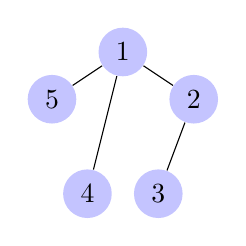
\begin{tikzpicture}
  [scale=.15,auto=left,every node/.style={circle,fill=blue!23}]
  \node (1) at (6,12) {1};
  \node (2) at (12,8)  {2};
  \node (3) at (9,0)  {3};
  \node (4) at (3,0)  {4};
  \node (5) at (0,8)  {5};
  
  \foreach \from/\to in {1/5,1/4,1/2,2/3}
    \draw (\from) -- (\to);

\end{tikzpicture}\hspace{6mm}
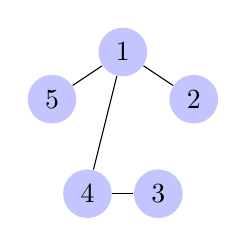
\begin{tikzpicture}
  [scale=.15,auto=left,every node/.style={circle,fill=blue!23}]
  \node (1) at (6,12) {1};
  \node (2) at (12,8)  {2};
  \node (3) at (9,0)  {3};
  \node (4) at (3,0)  {4};
  \node (5) at (0,8)  {5};
  
  \foreach \from/\to in {1/5,1/4,4/3,1/2}
    \draw (\from) -- (\to);

\end{tikzpicture}\hspace{6mm}
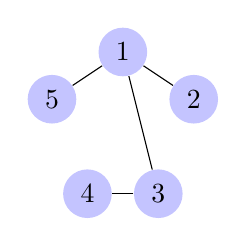
\begin{tikzpicture}
  [scale=.15,auto=left,every node/.style={circle,fill=blue!23}]
  \node (1) at (6,12) {1};
  \node (2) at (12,8)  {2};
  \node (3) at (9,0)  {3};
  \node (4) at (3,0)  {4};
  \node (5) at (0,8)  {5};
  
  \foreach \from/\to in {1/5,1/2,1/3,3/4}
    \draw (\from) -- (\to);

\end{tikzpicture}

\vspace{6mm}
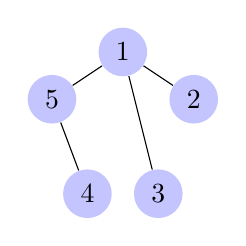
\begin{tikzpicture}
  [scale=.15,auto=left,every node/.style={circle,fill=blue!23}]
  \node (1) at (6,12) {1};
  \node (2) at (12,8)  {2};
  \node (3) at (9,0)  {3};
  \node (4) at (3,0)  {4};
  \node (5) at (0,8)  {5};
  
  \foreach \from/\to in {1/5,5/4,1/2,1/3}
    \draw (\from) -- (\to);

\end{tikzpicture}\hspace{6mm}
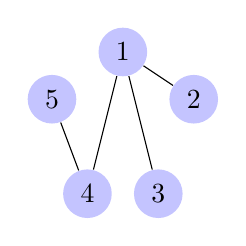
\begin{tikzpicture}
  [scale=.15,auto=left,every node/.style={circle,fill=blue!23}]
  \node (1) at (6,12) {1};
  \node (2) at (12,8)  {2};
  \node (3) at (9,0)  {3};
  \node (4) at (3,0)  {4};
  \node (5) at (0,8)  {5};
  
  \foreach \from/\to in {1/4,1/3,1/2,5/4}
    \draw (\from) -- (\to);

\end{tikzpicture}\hspace{6mm}
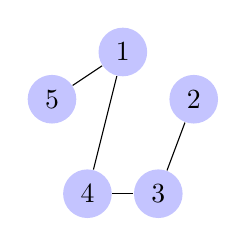
\begin{tikzpicture}
  [scale=.15,auto=left,every node/.style={circle,fill=blue!23}]
  \node (1) at (6,12) {1};
  \node (2) at (12,8)  {2};
  \node (3) at (9,0)  {3};
  \node (4) at (3,0)  {4};
  \node (5) at (0,8)  {5};
  
  \foreach \from/\to in {1/5,1/4,4/3,2/3}
    \draw (\from) -- (\to);

\end{tikzpicture}\hspace{6mm}
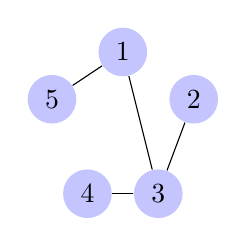
\begin{tikzpicture}
  [scale=.15,auto=left,every node/.style={circle,fill=blue!23}]
  \node (1) at (6,12) {1};
  \node (2) at (12,8)  {2};
  \node (3) at (9,0)  {3};
  \node (4) at (3,0)  {4};
  \node (5) at (0,8)  {5};
  
  \foreach \from/\to in {1/5,1/3,3/4,3/2}
    \draw (\from) -- (\to);

\end{tikzpicture}\hspace{6mm}
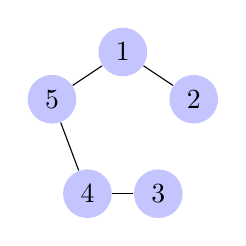
\begin{tikzpicture}
  [scale=.15,auto=left,every node/.style={circle,fill=blue!23}]
  \node (1) at (6,12) {1};
  \node (2) at (12,8)  {2};
  \node (3) at (9,0)  {3};
  \node (4) at (3,0)  {4};
  \node (5) at (0,8)  {5};
  
  \foreach \from/\to in {1/5,1/2,5/4,4/3}
    \draw (\from) -- (\to);

\end{tikzpicture}

\vspace{6mm}
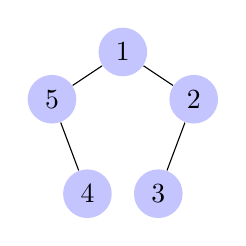
\begin{tikzpicture}
  [scale=.15,auto=left,every node/.style={circle,fill=blue!23}]
  \node (1) at (6,12) {1};
  \node (2) at (12,8)  {2};
  \node (3) at (9,0)  {3};
  \node (4) at (3,0)  {4};
  \node (5) at (0,8)  {5};
  
  \foreach \from/\to in {1/5,5/4,3/2,1/2}
    \draw (\from) -- (\to);

\end{tikzpicture}\hspace{6mm}
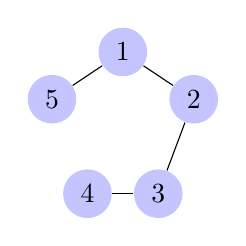
\begin{tikzpicture}
  [scale=.15,auto=left,every node/.style={circle,fill=blue!23}]
  \node (1) at (6,12) {1};
  \node (2) at (12,8)  {2};
  \node (3) at (9,0)  {3};
  \node (4) at (3,0)  {4};
  \node (5) at (0,8)  {5};
  
  \foreach \from/\to in {1/5,1/2,2/3,3/4}
    \draw (\from) -- (\to);

\end{tikzpicture}\hspace{6mm}
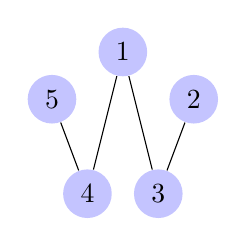
\begin{tikzpicture}
  [scale=.15,auto=left,every node/.style={circle,fill=blue!23}]
  \node (1) at (6,12) {1};
  \node (2) at (12,8)  {2};
  \node (3) at (9,0)  {3};
  \node (4) at (3,0)  {4};
  \node (5) at (0,8)  {5};
  
  \foreach \from/\to in {1/4,4/5,1/3,3/2}
    \draw (\from) -- (\to);

\end{tikzpicture}\hspace{6mm}
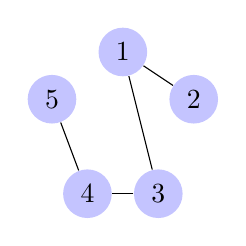
\begin{tikzpicture}
  [scale=.15,auto=left,every node/.style={circle,fill=blue!23}]
  \node (1) at (6,12) {1};
  \node (2) at (12,8)  {2};
  \node (3) at (9,0)  {3};
  \node (4) at (3,0)  {4};
  \node (5) at (0,8)  {5};
  
  \foreach \from/\to in {1/3,1/2,3/4,4/5}
    \draw (\from) -- (\to);

\end{tikzpicture}\hspace{6mm}
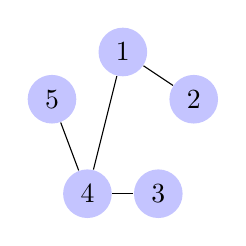
\begin{tikzpicture}
  [scale=.15,auto=left,every node/.style={circle,fill=blue!23}]
  \node (1) at (6,12) {1};
  \node (2) at (12,8)  {2};
  \node (3) at (9,0)  {3};
  \node (4) at (3,0)  {4};
  \node (5) at (0,8)  {5};
  
  \foreach \from/\to in {1/4,1/2,4/5,4/3}
    \draw (\from) -- (\to);

\end{tikzpicture}

\vspace{6mm}
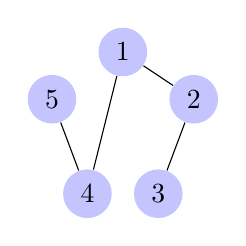
\begin{tikzpicture}
  [scale=.15,auto=left,every node/.style={circle,fill=blue!23}]
  \node (1) at (6,12) {1};
  \node (2) at (12,8)  {2};
  \node (3) at (9,0)  {3};
  \node (4) at (3,0)  {4};
  \node (5) at (0,8)  {5};
  
  \foreach \from/\to in {1/4,1/2,4/5,2/3}
    \draw (\from) -- (\to);

\end{tikzpicture}\hspace{6mm}
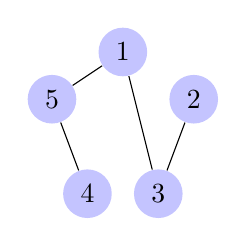
\begin{tikzpicture}
  [scale=.15,auto=left,every node/.style={circle,fill=blue!23}]
  \node (1) at (6,12) {1};
  \node (2) at (12,8)  {2};
  \node (3) at (9,0)  {3};
  \node (4) at (3,0)  {4};
  \node (5) at (0,8)  {5};
  
  \foreach \from/\to in {1/5,1/3,5/4,3/2}
    \draw (\from) -- (\to);

\end{tikzpicture}\hspace{6mm}
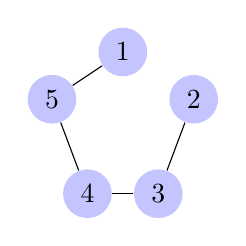
\begin{tikzpicture}
  [scale=.15,auto=left,every node/.style={circle,fill=blue!23}]
  \node (1) at (6,12) {1};
  \node (2) at (12,8)  {2};
  \node (3) at (9,0)  {3};
  \node (4) at (3,0)  {4};
  \node (5) at (0,8)  {5};
  
  \foreach \from/\to in {1/5,5/4,4/3,3/2}
    \draw (\from) -- (\to);

\end{tikzpicture}\hspace{6mm}
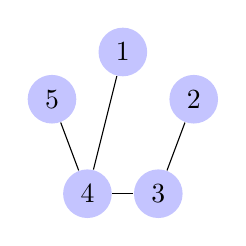
\begin{tikzpicture}
  [scale=.15,auto=left,every node/.style={circle,fill=blue!23}]
  \node (1) at (6,12) {1};
  \node (2) at (12,8)  {2};
  \node (3) at (9,0)  {3};
  \node (4) at (3,0)  {4};
  \node (5) at (0,8)  {5};
  
  \foreach \from/\to in {1/4,4/5,4/3,3/2}
    \draw (\from) -- (\to);

\end{tikzpicture}\hspace{6mm}
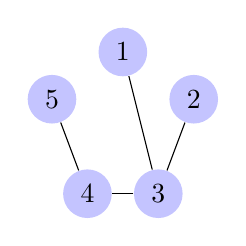
\begin{tikzpicture}
  [scale=.15,auto=left,every node/.style={circle,fill=blue!23}]
  \node (1) at (6,12) {1};
  \node (2) at (12,8)  {2};
  \node (3) at (9,0)  {3};
  \node (4) at (3,0)  {4};
  \node (5) at (0,8)  {5};
  
  \foreach \from/\to in {1/3,3/4,4/5,3/2}
    \draw (\from) -- (\to);

\end{tikzpicture}

\vspace{6mm}
\vspace{6mm}
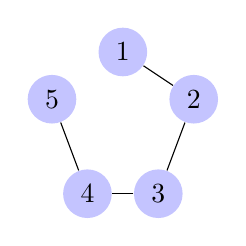
\begin{tikzpicture}
  [scale=.15,auto=left,every node/.style={circle,fill=blue!23}]
  \node (1) at (6,12) {1};
  \node (2) at (12,8)  {2};
  \node (3) at (9,0)  {3};
  \node (4) at (3,0)  {4};
  \node (5) at (0,8)  {5};
  
  \foreach \from/\to in {1/2,2/3,3/4,4/5}
    \draw (\from) -- (\to);

\end{tikzpicture}\hspace{6mm}
\end{center}


\newpage
\textbf{5c.} Compute the Laplacian spectrum of \(S_4\). 

\vspace{4mm}
\textit{Solution.} We first observe that 
\[L(G)= 
\begin{bmatrix} 
3 & -1 & -1 & -1 \\
-1& 1 &0&0\\
-1&0&1&0\\
-1&0&0&1
\end{bmatrix}
\]
To compute the eigenvalues, we find the values of \(\lambda\) such that \(\det(L(G)-\lambda I)=0\). Using mathematic, we find the characteristic function and also we find the roots of this characteristic function. 
\begin{verbatim}
In[5]:= G = {
  {3 - x, -1, -1, -1},
  {-1, 1 - x, 0, 0},
  {-1, 0, 1 - x, 0},
  {-1, 0, 0, 1 - x}
 }

Out[5]= {{3 - x, -1, -1, -1}, {-1, 1 - x, 0, 0}, {-1, 0, 1 - x, 
  0}, {-1, 0, 0, 1 - x}}

In[6]:= Det[G]

Out[6]= -4 x + 9 x^2 - 6 x^3 + x^4

In[7]:= Solve[-4 x + 9 x^2 - 6 x^3 + x^4 == 0, x]

Out[7]= {{x -> 0}, {x -> 1}, {x -> 1}, {x -> 4}}
\end{verbatim}
Thus, the eigenvalues \(\lambda\)s are \(\{ 4,1,1,0\}\). Therefore, the spectrum of \(G\) is 
\[
s(G) = (4,1,1,0).
\]

\vspace{6mm}
\textbf{7c.} Confirm that the algebraic connectivity \(a(G)\leq \kappa(G) \) for \(G=S_4\). 

\vspace{3mm} 
\textit{Solution.} Notice that the connectivity of \(\kappa(S_4)=1\) since if we remove the center vertex and its adjacent edges, the resulting graph will be disconnected. Also notice that the algebraic connectivity \(a(G)=1\). This is defined as the second smallest eigenvalue of the Laplacian matrix of \(G\). We computed this in problem \textbf{5c}, and showed that \(a(G)=1\). And since \(1\leq1 \Rightarrow\) \(a(S_4) \leq \kappa(S_4) \qed\) 

\newpage
\textbf{33.} Prove that the graphs in Figure 9.13 are not isomorphic but are isospectral. 

\vspace{3mm}

\textit{Proof.} Let \(G=(V,E)\) and \(H= (V',E')\) be the first and second graphs in figure 9.13 respectively. To show these graphs are not isomorphic we will assume they are and show a contradiction. Suppose \(G\cong H\). Then there exist a bijection \(f:V\rightarrow V'\) such that \(\{u,v\} \in E\) if and only if \( \{f(u),f(v)\}  \in E'\). We also know that the degree sequences of both graphs must be equal since the degree sequence is graph invariant. It follows from this that for each vertex \(v \in V\), the degree of \(v\) must equal the degree of \( f(v)\in V' \). (\(d(v)=d(f(v)\)). Next, observe from the figure that both \(G\) and \(H\) have precisely one vertex with a degree of 3. We will denote this vertex as \(\hat v \in V\) and \(f(\hat v) \in V'\). Thus \(d(\hat v) = d(f(\hat v) = 3\). Next we observe that each graph has exactly three vertices of degree four. We will denote these vertices in \(G\) as \(a,b,c\) and in \(H\) as \(f(a),f(b),f(c)\). Next we observe that \(\hat v \in G\) is adjacent to the three vertices of degree four. Thus, the edges, \( \{\hat v, a\}, \{\hat v, b\}, \{\hat v,c\} \in E\). Since \(f\) is an isomorphism then the edges \(\{f(\hat v), f(a)\}, \{f(\hat v), f(b)\}, \{f(\hat v),f(c)\}\) must be in the edge set of \(H\), \(E'\). And since we know that the degree of the vertices \(a,b,c\) is four, then the degrees of \(f(a),f(b),f(c)\) must also be four. Thus \(f(\hat v)\) must also adjacent to precisely three vertices of degree four in \(H\). \(\rightarrow\!\leftarrow\) But this is clearly not the case since we see that the only vertex of degree 3 in \(H\) is adjacent to two vertices of degree 5 and one vertex of degree four. Thus, \(G\) and \(H\) are not isomorphic. \(\qed\)


\vspace{3mm} To show that \(G\) and \(H\) are isospectral we will use Mathematica to compute the spectrum of both graphs. 
\begin{verbatim}
In[10]:= G = {  {4, -1, 0, -1, -1, 0, -1},
  {-1, 5, -1, -1, -1, -1, 0},
  {0, -1, 4, -1, -1, 0, -1},
  {-1, -1, -1, 5, -1, -1, 0},
  {-1, -1, -1, -1, 5, -1, 0},
  {0, -1, 0, -1, -1, 4, -1},
  {-1, 0, -1, 0, 0, -1, 3} }
Out[10]= {{4, -1, 0, -1, -1, 0, -1}, {-1, 5, -1, -1, -1, -1, 
  0}, {0, -1, 4, -1, -1, 0, -1}, {-1, -1, -1, 5, -1, -1, 
  0}, {-1, -1, -1, -1, 5, -1, 0}, {0, -1, 0, -1, -1, 4, -1}, {-1, 
  0, -1, 0, 0, -1, 3}}
In[11]:= Eigenvalues[G]
Out[11]= {7, 6, 6, 4, 4, 3, 0}
In[14]:= 
H = {  {5, -1, -1, -1, 0, -1, -1},
  {-1, 4, -1, 0, -1, 0, -1},
  {-1, -1, 4, -1, 0, -1, 0},
  {-1, 0, -1, 5, -1, -1, -1},
  {0, -1, 0, -1, 3, -1, 0},
  {-1, 0, -1, -1, -1, 5, -1},
  {-1, -1, 0, -1, 0, -1, 4} }
Out[14]= {{5, -1, -1, -1, 0, -1, -1}, {-1, 4, -1, 0, -1, 
  0, -1}, {-1, -1, 4, -1, 0, -1, 0}, {-1, 0, -1, 
  5, -1, -1, -1}, {0, -1, 0, -1, 3, -1, 0}, {-1, 0, -1, -1, -1, 
  5, -1}, {-1, -1, 0, -1, 0, -1, 4}}
In[15]:= Eigenvalues[H]
Out[15]= {7, 6, 6, 4, 4, 3, 0}
\end{verbatim}
Thus we have shown that \(s(G)=\{7,6,6,4,4,3,0\}\) and \(s(H)=\{7,6,6,4,4,3,9\}\). Since \(s(G)=s(H)\), then \(G\) and \(H\) are \textit{isospectral}. \(\qed\)

















\end{document}
